\begin{enumerate}[label=\thesubsection.\arabic*, ref=\thesubsection.\theenumi]
\item
If tangents $PA$ and $PB$ drawn from an external point $P$ to a circle with centre $O$ are inclined to each other at an angle of $80^\circ$, then $\angle POA$ is equal to
\hfill (10, 2025)
\begin{enumerate}
	\begin{multicols}{4}
    \item $40^\circ$
    \item $50^\circ$
    \item $60^\circ$
    \item $80^\circ$
	\end{multicols}
\end{enumerate}
\solution
Take the centre $\vec{O} = \myvec{0 \\ 0}$ as the origin and $\vec{P} = \myvec{d \\ 0}$ on the $x$-axis. Let $r$ be the radius and $\phi = \angle POA$. The points of contact are symmetric about $OP$, so
\begin{align}
	\vec{A} = r\myvec{\cos\phi \\ \sin\phi}, \quad \vec{B} = r\myvec{\cos\phi \\ -\sin\phi}
\end{align}
The radius is perpendicular to the tangent at the point of contact,
\begin{align}
	\brak{\vec{A}-\vec{O}}^{\top}\brak{\vec{A}-\vec{P}} = 0 \implies \norm{\vec{A}}^2 = \vec{A}^{\top}\vec{P}
	\implies r^2 = rd\cos\phi \implies r = d\cos\phi
\end{align}
Hence the direction vectors of the tangents $PA$ and $PB$ are
\begin{align}
	\vec{A}-\vec{P} &= d\myvec{\cos^2\phi - 1 \\ \sin\phi\cos\phi} = d\sin\phi\myvec{-\sin\phi \\ \cos\phi}
	\\
	\vec{B}-\vec{P} &= d\myvec{\cos^2\phi - 1 \\ -\sin\phi\cos\phi} = d\sin\phi\myvec{-\sin\phi \\ -\cos\phi}
\end{align}
The unit direction vectors are $\vec{m}_1 = \myvec{-\sin\phi \\ \cos\phi}$ and $\vec{m}_2 = \myvec{-\sin\phi \\ -\cos\phi}$, so the angle between the tangents satisfies
\begin{align}
	\cos\angle APB = \vec{m}_1^{\top}\vec{m}_2 = \sin^2\phi - \cos^2\phi = -\cos 2\phi
\end{align}
Given $\angle APB = 80^\circ$,
\begin{align}
	\cos 2\phi = -\cos 80^\circ = \cos 100^\circ \implies \phi = 50^\circ
	\implies \angle POA = 50^\circ \quad \brak{\text{Option B}}
\end{align}
Taking $r = 2$, we get $d = \frac{r}{\cos 50^\circ} \approx 3.11$ and the points
\begin{align}
	\vec{O} = \myvec{0 \\ 0}, \quad \vec{P} = \myvec{3.11 \\ 0}, \quad
	\vec{A} = \myvec{1.29 \\ 1.53}, \quad \vec{B} = \myvec{1.29 \\ -1.53}
\end{align}
The following code verifies the solution
\begin{lstlisting}[frame=single, basicstyle=\rmfamily, escapeinside={(*@}{@*)}]
(*@\makebox[\dimexpr\linewidth-2\fboxsep-2\fboxrule\relax][c]{10/codes/1.py}@*)
\end{lstlisting}
The following code generates \figref{fig:CBSE25S2-q1}.
\begin{lstlisting}[frame=single, basicstyle=\rmfamily, escapeinside={(*@}{@*)}]
(*@\makebox[\dimexpr\linewidth-2\fboxsep-2\fboxrule\relax][c]{10/codes/1plot.py}@*)
\end{lstlisting}
\begin{figure}[H]
	\centering
	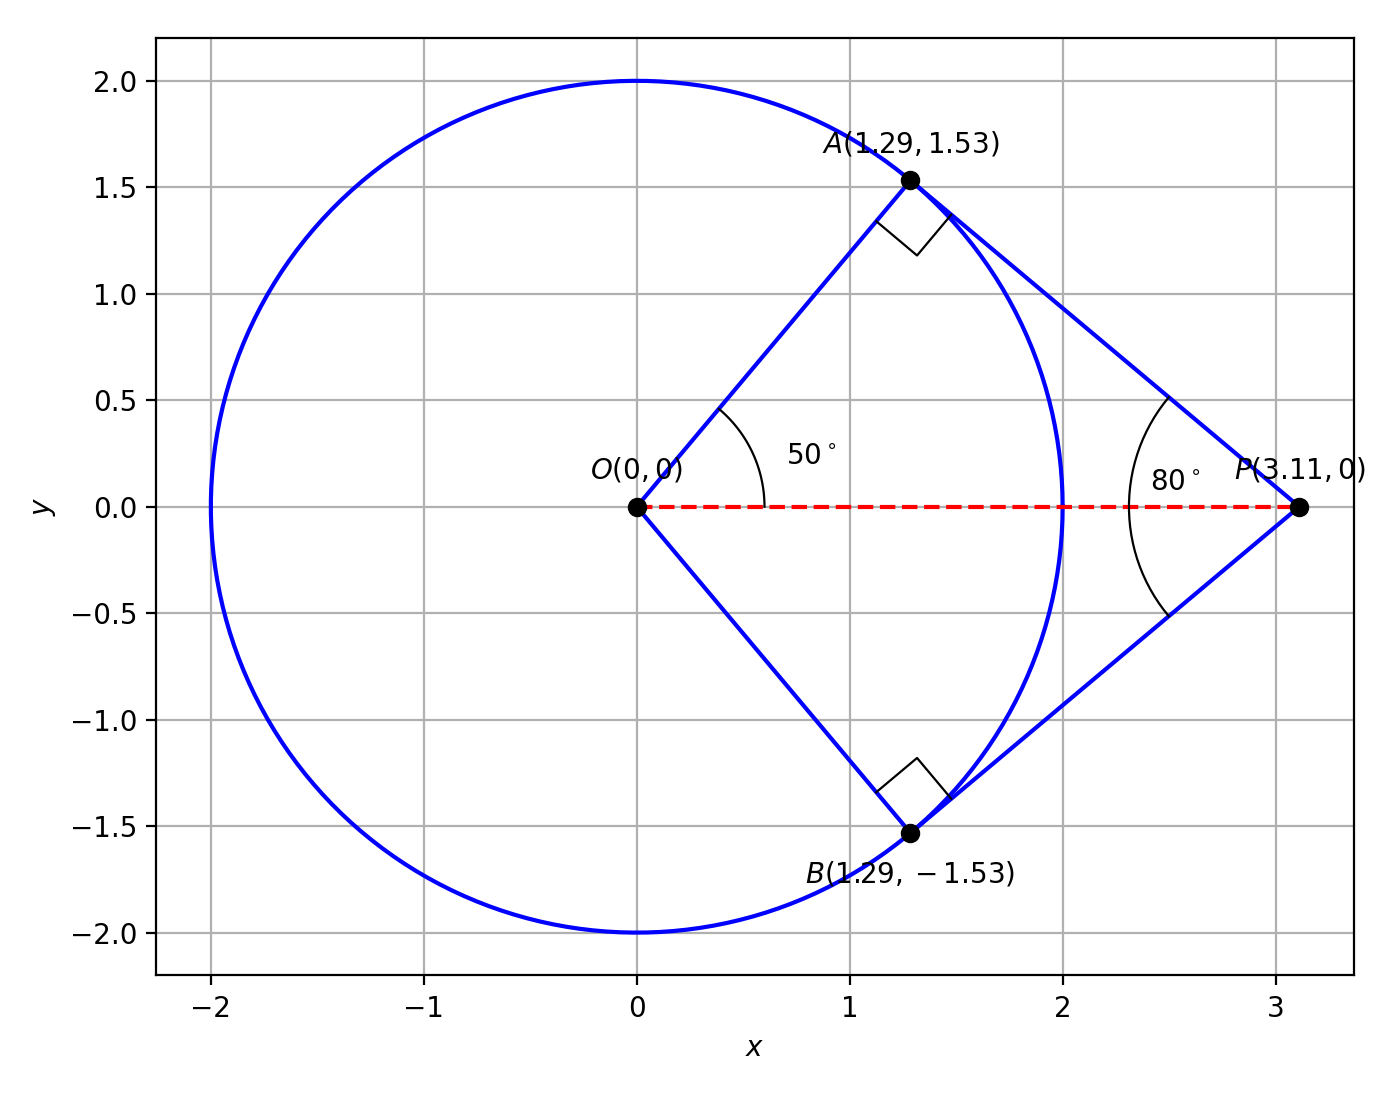
\includegraphics[width=0.6\linewidth]{figs/q1.png}
	\caption{Tangents $PA$ and $PB$ plotted from the coordinates of $\vec{O}$, $\vec{P}$, $\vec{A}$, $\vec{B}$}
	\label{fig:CBSE25S2-q1}
\end{figure}

\item
Two vertices of $\triangle PQR$ are $P\brak{-1,5}$ and $Q\brak{5,2}$. The coordinates of the point $R$ on $PQ$ which divides $PQ$ in the ratio $2:1$ are
\hfill (10, 2025)
\begin{enumerate}
	\begin{multicols}{4}
    \item $\brak{3,-3}$
    \item $\brak{5,5}$
    \item $\brak{3,3}$
    \item $\brak{5,1}$
	\end{multicols}
\end{enumerate}

\solution
The point $\vec{R}$ divides the segment joining $\vec{P} = \myvec{-1 \\ 5}$ and $\vec{Q} = \myvec{5 \\ 2}$ internally in the ratio $m:n = 2:1$. By the section formula,
\begin{align}
	\vec{R} = \frac{m\vec{Q} + n\vec{P}}{m+n} = \frac{2\myvec{5 \\ 2} + 1\myvec{-1 \\ 5}}{2+1} = \frac{1}{3}\myvec{9 \\ 9} = \myvec{3 \\ 3} \quad \brak{\text{Option C}}
\end{align}
The following code verifies the solution
\begin{lstlisting}[frame=single, basicstyle=\rmfamily, escapeinside={(*@}{@*)}]
(*@\makebox[\dimexpr\linewidth-2\fboxsep-2\fboxrule\relax][c]{10/codes/4.py}@*)
\end{lstlisting}
The following code generates \figref{fig:CBSE25S2-q4}.
\begin{lstlisting}[frame=single, basicstyle=\rmfamily, escapeinside={(*@}{@*)}]
(*@\makebox[\dimexpr\linewidth-2\fboxsep-2\fboxrule\relax][c]{10/codes/4plot.py}@*)
\end{lstlisting}
\begin{figure}[H]
	\centering
	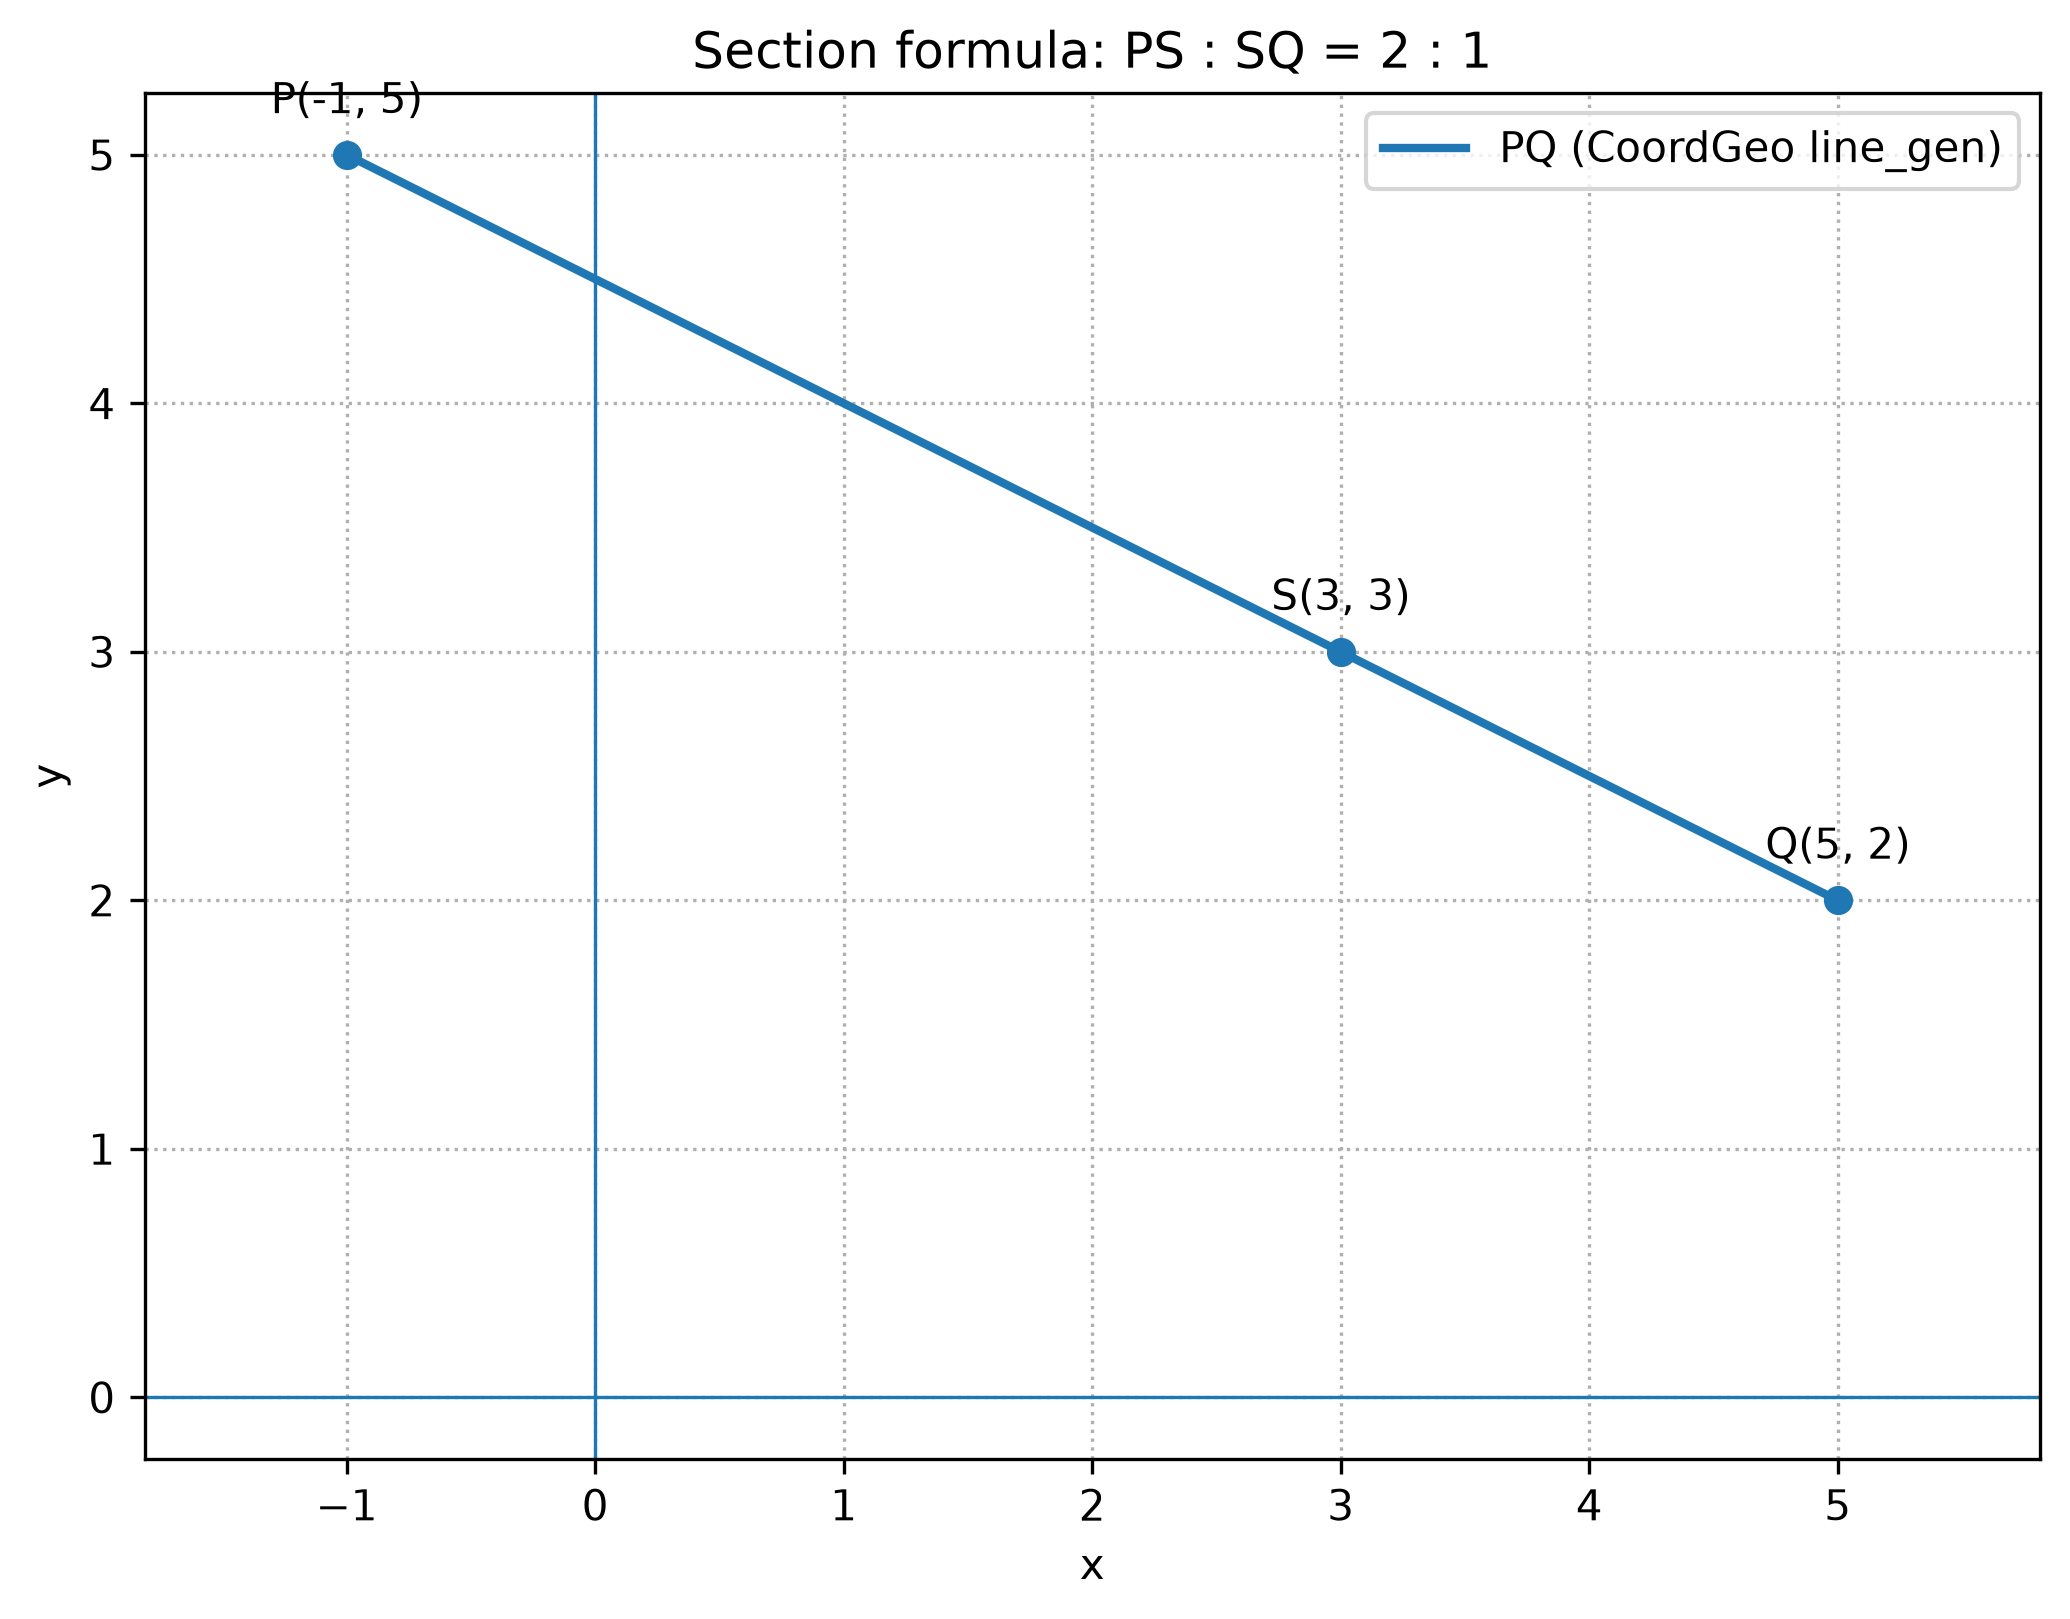
\includegraphics[width=0.5\linewidth]{figs/q4.png}
	\caption{Point $R$ dividing $PQ$ in the ratio $2:1$}
	\label{fig:CBSE25S2-q4}
\end{figure}

\item
If $\sin 4\theta = \frac{\sqrt{3}}{2}$, then $\frac{\theta}{3}$ is equal to
\hfill (10, 2025)
\begin{enumerate}
	\begin{multicols}{4}
    \item $60^\circ$
    \item $20^\circ$
    \item $15^\circ$
    \item $5^\circ$
	\end{multicols}
\end{enumerate}

\solution
Taking the principal (acute) value,
\begin{align}
	4\theta = \sin^{-1}\brak{\frac{\sqrt{3}}{2}} = 60^\circ
	\implies \theta = 15^\circ
	\implies \frac{\theta}{3} = 5^\circ \quad \brak{\text{Option D}}
\end{align}
The following code verifies the solution
\begin{lstlisting}[frame=single, basicstyle=\rmfamily, escapeinside={(*@}{@*)}]
(*@\makebox[\dimexpr\linewidth-2\fboxsep-2\fboxrule\relax][c]{10/codes/5.py}@*)
\end{lstlisting}

\item
The zeroes of the polynomial $p\brak{y} = 7y^2 - \frac{11}{3}y - \frac{2}{3}$ are
\hfill (10, 2025)
\begin{enumerate}
    \begin{multicols}{4}
        \item $\displaystyle -\frac{2}{3},-\frac{1}{7}$
        \item $\displaystyle -\frac{2}{7},-\frac{1}{3}$
        \item $\displaystyle \frac{2}{3},\frac{1}{7}$
        \item $\displaystyle \frac{2}{3},-\frac{1}{7}$
    \end{multicols}
\end{enumerate}

\solution
Multiplying by $3$, the zeroes of $p$ are the zeroes of
\begin{align}
	g\brak{y} = 21y^2 - 11y - 2, \quad g^{\prime}\brak{y} = 42y - 11
\end{align}
To find a zero iteratively, expand $g$ about the current estimate $y_n$ to first order and require the next estimate $y_{n+1}$ to be a zero,
\begin{align}
	g\brak{y_{n+1}} \approx g\brak{y_n} + g^{\prime}\brak{y_n}\brak{y_{n+1} - y_n} = 0
\end{align}
which gives the difference equation (Newton--Raphson iteration)
\begin{align}
	y_{n+1} = y_n - \frac{g\brak{y_n}}{g^{\prime}\brak{y_n}} = y_n - \frac{21y_n^2 - 11y_n - 2}{42y_n - 11}
\end{align}
with the initial value $y_0$.
Starting from $y_0 = 0.7$ and $y_0 = -0.2$, the iterations converge to
\begin{align}
	y = \frac{2}{3}, \quad y = -\frac{1}{7} \quad \brak{\text{Option D}}
\end{align}
which agree with the factorisation $g\brak{y} = \brak{3y-2}\brak{7y+1}$. The following code verifies the solution
\begin{lstlisting}[frame=single, basicstyle=\rmfamily, escapeinside={(*@}{@*)}]
(*@\makebox[\dimexpr\linewidth-2\fboxsep-2\fboxrule\relax][c]{10/codes/6.c}@*)
\end{lstlisting}
The following code generates \figref{fig:CBSE25S2-q6}.
\begin{lstlisting}[frame=single, basicstyle=\rmfamily, escapeinside={(*@}{@*)}]
(*@\makebox[\dimexpr\linewidth-2\fboxsep-2\fboxrule\relax][c]{10/codes/6plot.py}@*)
\end{lstlisting}
\begin{figure}[H]
	\centering
	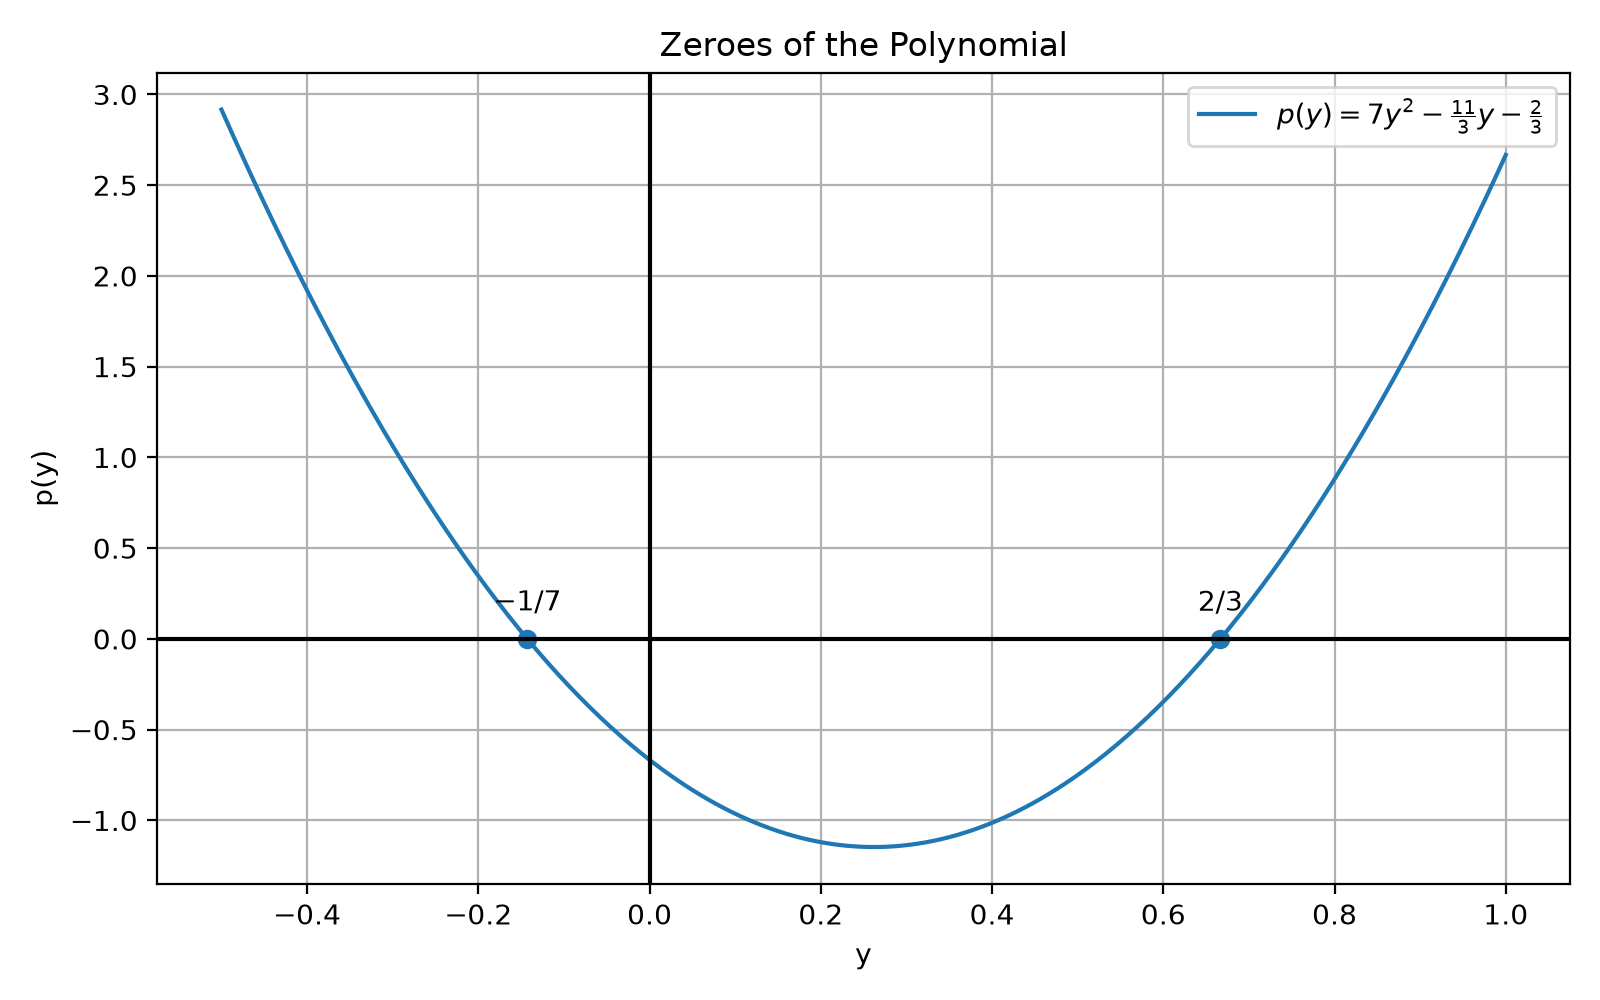
\includegraphics[width=0.6\linewidth]{figs/q6.png}
	\caption{Graph of $p\brak{y}$ and its zeroes}
	\label{fig:CBSE25S2-q6}
\end{figure}

\item
$AOBC$ is a rectangle whose three vertices are $A\brak{0,2}$, $O\brak{0,0}$ and $B\brak{4,0}$. The square of the length of its diagonal is
\hfill (10, 2025)
\begin{enumerate}
	\begin{multicols}{4}
    \item $36$
    \item $20$
    \item $16$
    \item $4$
	\end{multicols}
\end{enumerate}

\solution
The fourth vertex is $C\brak{4,2}$ and the diagonal is $AB$. With $\vec{A} = \myvec{0\\2}$, $\vec{B} = \myvec{4\\0}$,
\begin{align}
	\vec{B} - \vec{A} = \myvec{4 \\ -2}, \qquad
	\norm{\vec{B}-\vec{A}}^2 = \brak{\vec{B}-\vec{A}}^{\top}\brak{\vec{B}-\vec{A}} = 16 + 4 = 20 \quad \brak{\text{Option B}}
\end{align}
The following code verifies the solution
\begin{lstlisting}[frame=single, basicstyle=\rmfamily, escapeinside={(*@}{@*)}]
(*@\makebox[\dimexpr\linewidth-2\fboxsep-2\fboxrule\relax][c]{10/codes/8.py}@*)
\end{lstlisting}
The following code generates \figref{fig:CBSE25S2-q8}.
\begin{lstlisting}[frame=single, basicstyle=\rmfamily, escapeinside={(*@}{@*)}]
(*@\makebox[\dimexpr\linewidth-2\fboxsep-2\fboxrule\relax][c]{10/codes/8plot.py}@*)
\end{lstlisting}
\begin{figure}[H]
	\centering
	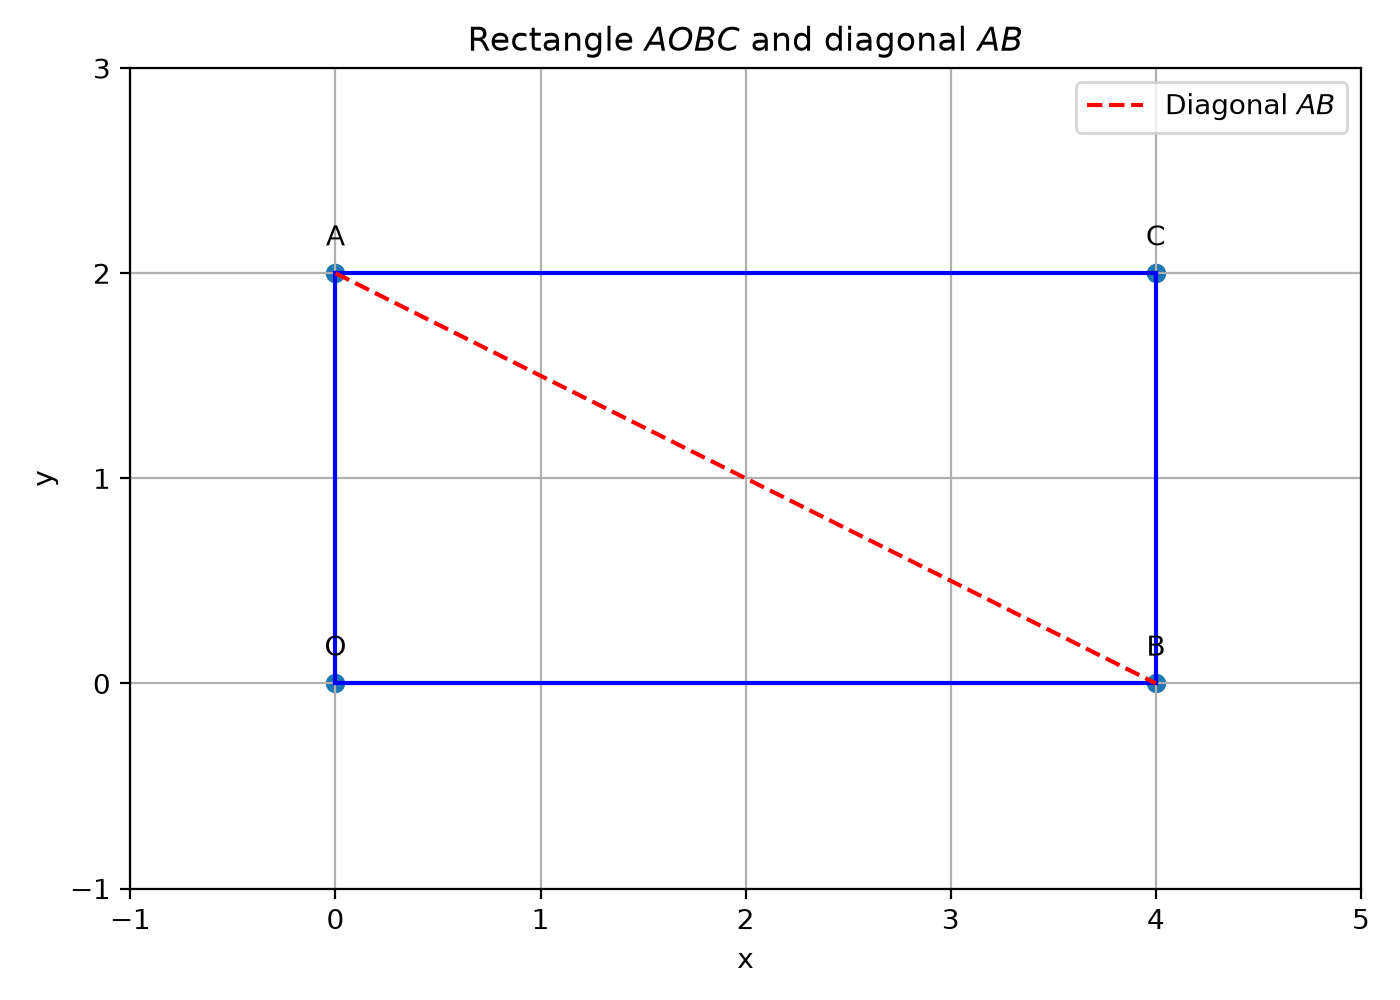
\includegraphics[width=0.55\linewidth]{figs/q8.png}
	\caption{Rectangle $AOBC$ and its diagonals}
	\label{fig:CBSE25S2-q8}
\end{figure}

\item
A die is thrown once. The probability of getting a number which is not a factor of $36$ is
\hfill (10, 2025)
\begin{enumerate}
	\begin{multicols}{4}
    \item $\frac{1}{2}$
    \item $\frac{2}{3}$
    \item $\frac{1}{6}$
    \item $\frac{5}{6}$
	\end{multicols}
\end{enumerate}

\solution
Let $X$ be the number on the upper face of a fair die. Its pmf is
\begin{table}[H]
	\centering
	\begin{tabular}{|c|c|c|c|c|c|c|}
		\hline
		$x$ & $1$ & $2$ & $3$ & $4$ & $5$ & $6$ \\ \hline
		$p_X\brak{x}$ & $\frac{1}{6}$ & $\frac{1}{6}$ & $\frac{1}{6}$ & $\frac{1}{6}$ & $\frac{1}{6}$ & $\frac{1}{6}$ \\ \hline
	\end{tabular}
	\caption{pmf of the number on a fair die}
	\label{tab:CBSE25S2-q10}
\end{table}
Since $36 = 1\times36 = 2\times18 = 3\times12 = 4\times9 = 6\times6$, the numbers $1,2,3,4,6$ are factors of $36$ and the event $E$ (``not a factor of $36$'') is $E = \cbrak{5}$. The probability of an event is the sum of the pmf over its outcomes,
\begin{align}
	\pr{E} = \sum_{x \in E} p_X\brak{x} = p_X\brak{5} = \frac{1}{6} \quad \brak{\text{Option C}}
\end{align}
The following program simulates $10^6$ throws of the die and compares the relative frequencies with the pmf and with $\pr{E}$
\begin{lstlisting}[frame=single, basicstyle=\rmfamily, escapeinside={(*@}{@*)}]
(*@\makebox[\dimexpr\linewidth-2\fboxsep-2\fboxrule\relax][c]{10/codes/10.c}@*)
\end{lstlisting}
The following code makes a stem plot of the simulated relative frequencies and the pmf, see \figref{fig:CBSE25S2-q10}.
\begin{lstlisting}[frame=single, basicstyle=\rmfamily, escapeinside={(*@}{@*)}]
(*@\makebox[\dimexpr\linewidth-2\fboxsep-2\fboxrule\relax][c]{10/codes/10plot.py}@*)
\end{lstlisting}
\begin{figure}[H]
	\centering
	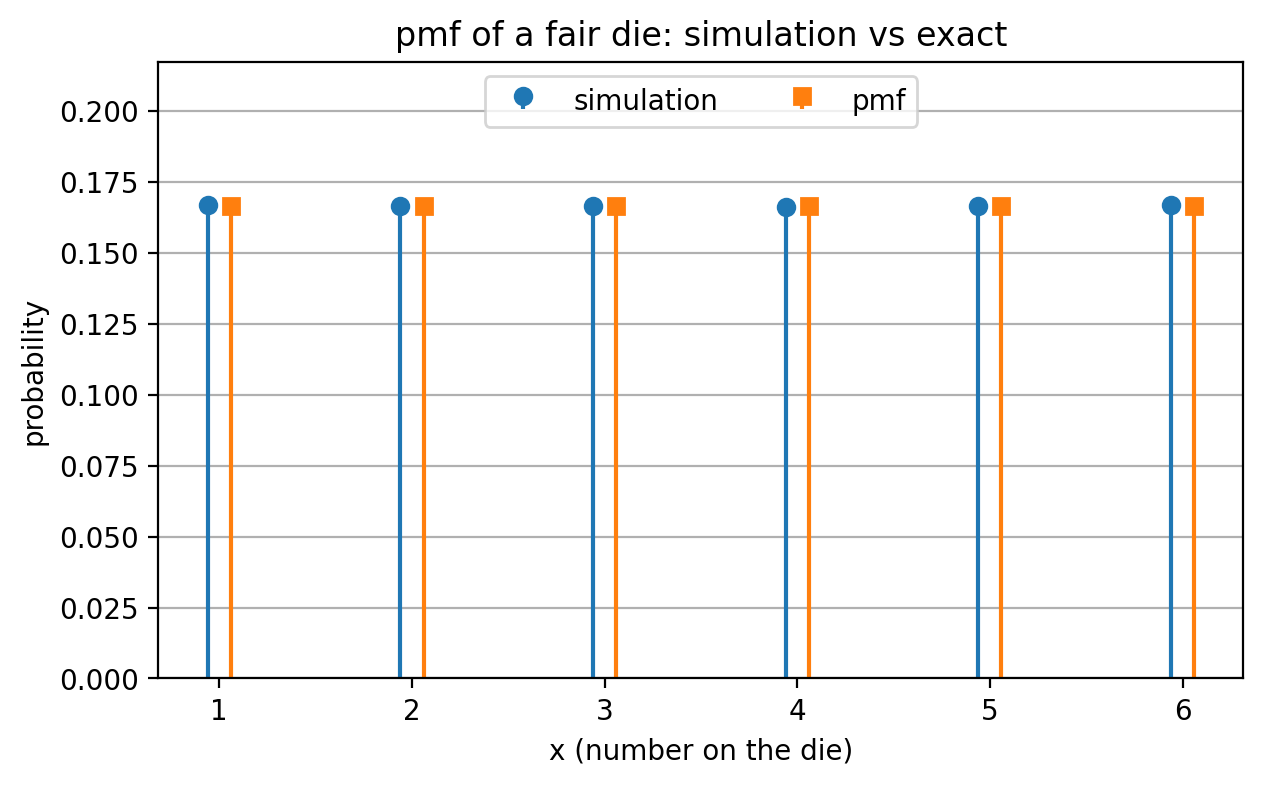
\includegraphics[width=0.8\linewidth]{figs/q10.png}
	\caption{Stem plot of the simulated relative frequencies and the pmf of a fair die}
	\label{fig:CBSE25S2-q10}
\end{figure}

\item
In the figure, $\angle BAC = 90^\circ$ and $AD \perp BC$. If $BC = 16$ cm and $DC = 4$ cm, then $AC = x$ is equal to
\hfill (10, 2025)
\begin{enumerate}
    \begin{multicols}{4}
        \item $4\text{ cm}$
        \item $5\text{ cm}$
        \item $8\text{ cm}$
        \item $3\text{ cm}$
    \end{multicols}
\end{enumerate}
\solution
Take $\vec{B} = \myvec{0\\0}$, $\vec{C} = \myvec{16\\0}$. Then $BD = 16-4 = 12$, so $\vec{D} = \myvec{12\\0}$ and, since $AD \perp BC$, $\vec{A} = \myvec{12\\h}$. As $\angle BAC = 90^\circ$,
\begin{align}
	\brak{\vec{B}-\vec{A}}^{\top}\brak{\vec{C}-\vec{A}} &= 0
	\\
	\myvec{-12 & -h}\myvec{4 \\ -h} = -48 + h^2 &= 0 \implies h^2 = 48
\end{align}
Hence,
\begin{align}
	x^2 = \norm{\vec{C}-\vec{A}}^2 = 4^2 + h^2 = 64 \implies x = 8 \text{ cm} \quad \brak{\text{Option C}}
\end{align}
The following code verifies the solution
\begin{lstlisting}[frame=single, basicstyle=\rmfamily, escapeinside={(*@}{@*)}]
(*@\makebox[\dimexpr\linewidth-2\fboxsep-2\fboxrule\relax][c]{10/codes/11.py}@*)
\end{lstlisting}
The following code generates \figref{fig:CBSE25S2-q11}.
\begin{lstlisting}[frame=single, basicstyle=\rmfamily, escapeinside={(*@}{@*)}]
(*@\makebox[\dimexpr\linewidth-2\fboxsep-2\fboxrule\relax][c]{10/codes/11plot.py}@*)
\end{lstlisting}
\begin{figure}[H]
	\centering
	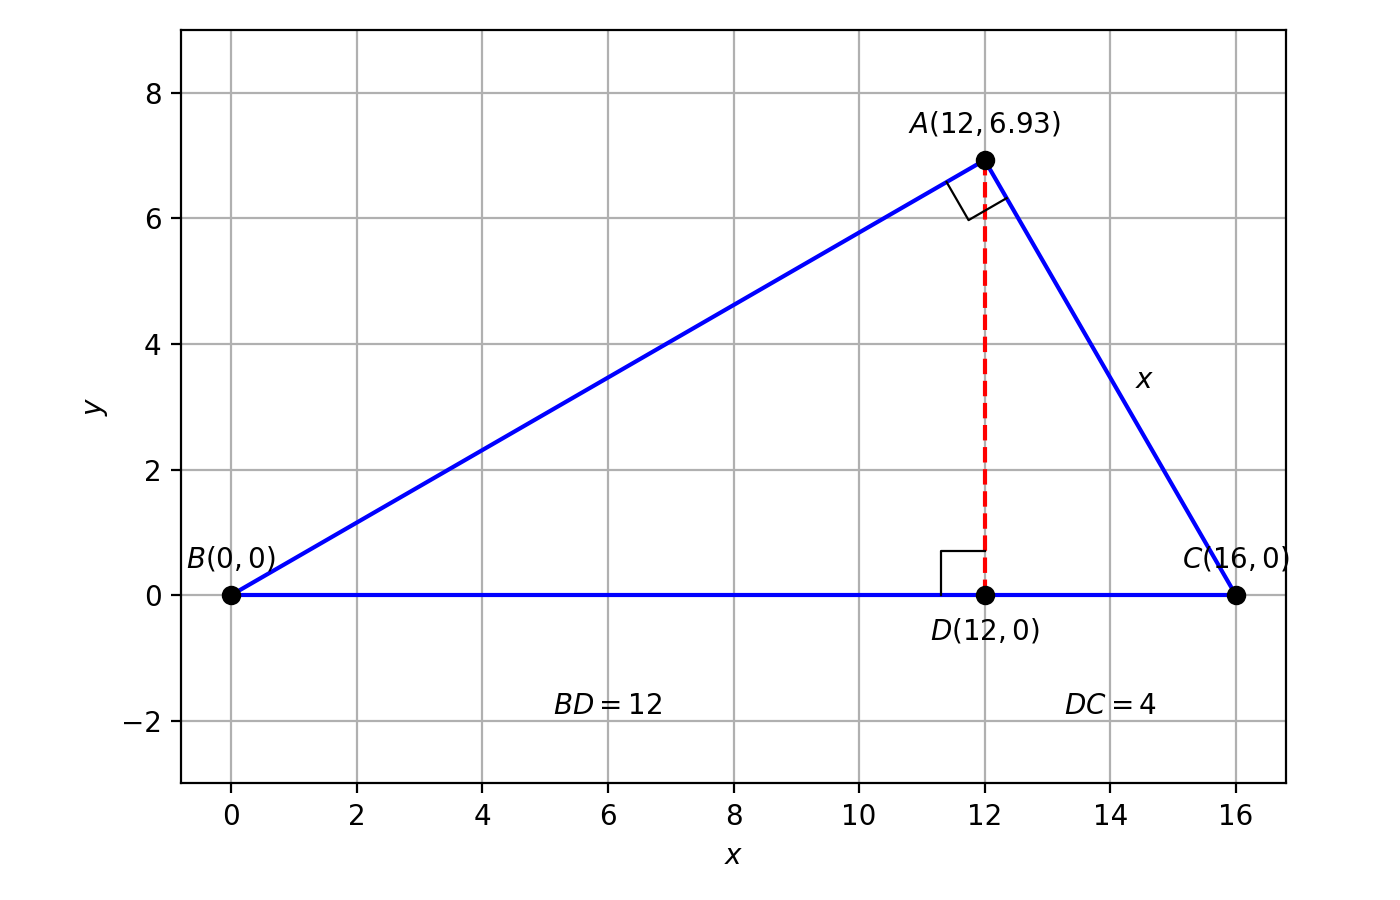
\includegraphics[width=0.6\linewidth]{figs/q11.png}
	\caption{Right triangle $ABC$ with altitude $AD$, plotted from the coordinates of $\vec{B}$, $\vec{C}$, $\vec{D}$, $\vec{A}$}
	\label{fig:CBSE25S2-q11}
\end{figure}

\item
The mid-point of the line segment joining $\brak{a,4}$ and $\brak{2,2b}$ is $\brak{2,6}$. Then $a + b$ is equal to
\hfill (10, 2025)
\begin{enumerate}
    \begin{multicols}{4}
        \item $6$
        \item $7$
        \item $8$
        \item $16$
    \end{multicols}
\end{enumerate}

\solution
Let $\vec{P} = \myvec{a \\ 4}$, $\vec{Q} = \myvec{2 \\ 2b}$ and let $\vec{M} = \myvec{2 \\ 6}$ be the mid-point. The mid-point is the average of the end points, so
\begin{align}
	\vec{M} = \frac{\vec{P} + \vec{Q}}{2} \implies 2\vec{M} = \vec{P} + \vec{Q} = \myvec{a + 2 \\ 4 + 2b}
\end{align}
Separating the known entries from the unknown ones,
\begin{align}
	2\vec{M} = \myvec{2 \\ 4} + \myvec{a \\ 2b}
\end{align}
Let $\vec{C} = \myvec{2 \\ 4}$ be the known part. Then
\begin{align}
	\myvec{a \\ 2b} = 2\vec{M} - \vec{C}
\end{align}
The unknown vector can be written with the unknowns $a$ and $b$ themselves,
\begin{align}
	\myvec{a \\ 2b} = \vec{D}\myvec{a \\ b}, \qquad \vec{D} = \myvec{1 & 0 \\ 0 & 2}
\end{align}
so that $\vec{D}\myvec{a \\ b} = 2\vec{M} - \vec{C}$. The matrix $\vec{D}$ is diagonal with non-zero entries, hence invertible, and
\begin{align}
	\myvec{a \\ b} = \vec{D}^{-1}\brak{2\vec{M} - \vec{C}}, \qquad \vec{D}^{-1} = \myvec{1 & 0 \\ 0 & \frac{1}{2}}
\end{align}
We need $a + b = \myvec{1 & 1}\myvec{a \\ b}$, therefore
\begin{align}
	a + b = \myvec{1 & 1}\vec{D}^{-1}\brak{2\vec{M} - \vec{C}}
\end{align}
Substituting $2\vec{M} - \vec{C} = \myvec{4 \\ 12} - \myvec{2 \\ 4} = \myvec{2 \\ 8}$,
\begin{align}
	\myvec{a \\ b} = \myvec{1 & 0 \\ 0 & \frac{1}{2}}\myvec{2 \\ 8} = \myvec{2 \\ 4}
	\implies a + b = \myvec{1 & 1}\myvec{2 \\ 4} = 6 \quad \brak{\text{Option A}}
\end{align}
Check: for $\vec{P} = \myvec{2 \\ 4}$ and $\vec{Q} = \myvec{2 \\ 8}$ the mid-point is $\frac{1}{2}\myvec{4 \\ 12} = \myvec{2 \\ 6}$. The following code verifies the solution
\begin{lstlisting}[frame=single, basicstyle=\rmfamily, escapeinside={(*@}{@*)}]
(*@\makebox[\dimexpr\linewidth-2\fboxsep-2\fboxrule\relax][c]{10/codes/15.py}@*)
\end{lstlisting}
The following code generates \figref{fig:CBSE25S2-q15}.
\begin{lstlisting}[frame=single, basicstyle=\rmfamily, escapeinside={(*@}{@*)}]
(*@\makebox[\dimexpr\linewidth-2\fboxsep-2\fboxrule\relax][c]{10/codes/15plot.py}@*)
\end{lstlisting}
\begin{figure}[H]
	\centering
	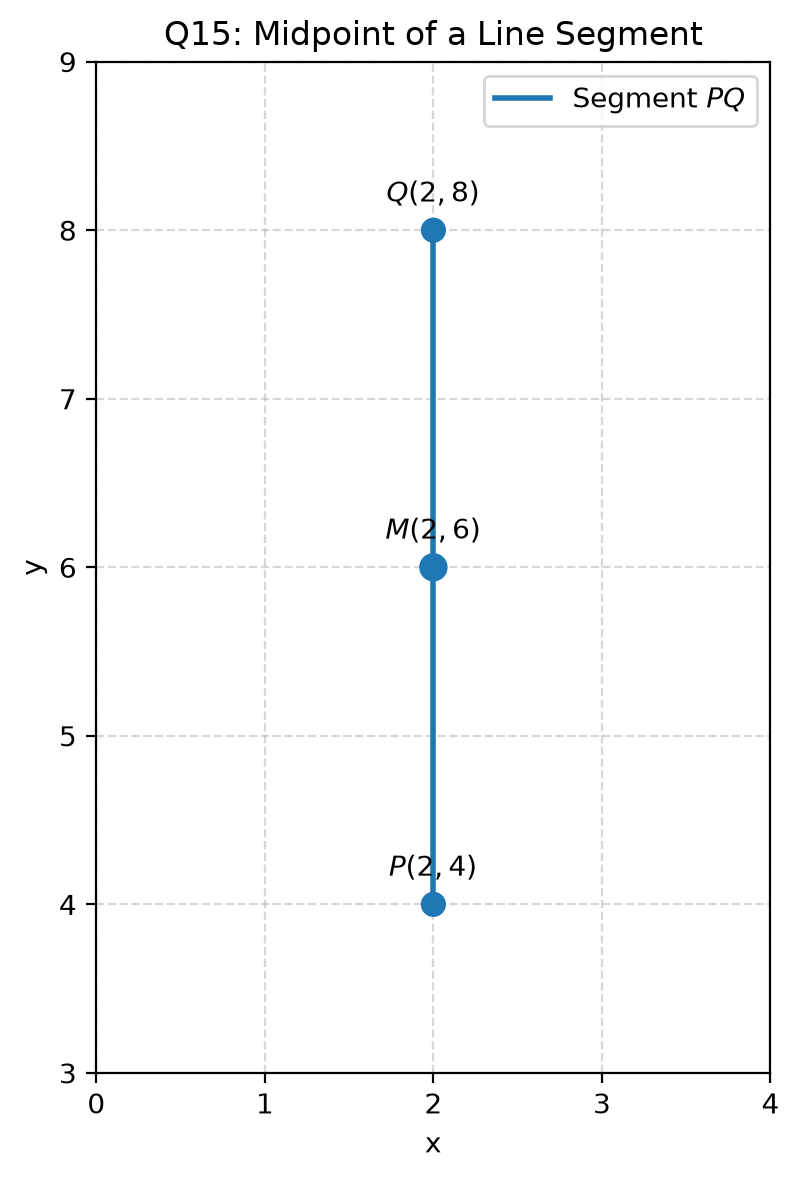
\includegraphics[width=0.45\linewidth]{figs/q15.png}
	\caption{Segment $PQ$ and its mid-point $M$}
	\label{fig:CBSE25S2-q15}
\end{figure}

\item
If $\alpha$ and $\beta$ are the zeroes of the polynomial $x^2 - 2x - 1$, find the value of $\frac{1}{2\alpha} + \frac{1}{2\beta} + 3\alpha\beta$.
\hfill (10, 2025)

\solution
Let $f\brak{x} = x^2 - 2x - 1$, so $f^{\prime}\brak{x} = 2x - 2$. Expanding $f$ about the current estimate $x_n$ to first order and requiring $f\brak{x_{n+1}} = 0$,
\begin{align}
	f\brak{x_n} + f^{\prime}\brak{x_n}\brak{x_{n+1} - x_n} = 0
\end{align}
gives the difference equation (Newton--Raphson iteration)
\begin{align}
	x_{n+1} = x_n - \frac{f\brak{x_n}}{f^{\prime}\brak{x_n}} = x_n - \frac{x_n^2 - 2x_n - 1}{2x_n - 2}
\end{align}
Starting from $x_0 = 2.5$ and $x_0 = -0.5$ gives
\begin{align}
	\alpha = 1 + \sqrt{2}, \quad \beta = 1 - \sqrt{2}
\end{align}
From the sum and product of zeroes, $\alpha + \beta = 2$ and $\alpha\beta = -1$, so
\begin{align}
	\frac{1}{2\alpha} + \frac{1}{2\beta} + 3\alpha\beta = \frac{\alpha+\beta}{2\alpha\beta} + 3\alpha\beta = \frac{2}{-2} - 3 = -4
\end{align}
The following code verifies the solution
\begin{lstlisting}[frame=single, basicstyle=\rmfamily, escapeinside={(*@}{@*)}]
(*@\makebox[\dimexpr\linewidth-2\fboxsep-2\fboxrule\relax][c]{10/codes/21.c}@*)
\end{lstlisting}
The following code generates \figref{fig:CBSE25S2-q21b}.
\begin{lstlisting}[frame=single, basicstyle=\rmfamily, escapeinside={(*@}{@*)}]
(*@\makebox[\dimexpr\linewidth-2\fboxsep-2\fboxrule\relax][c]{10/codes/21plot.py}@*)
\end{lstlisting}
\begin{figure}[H]
	\centering
	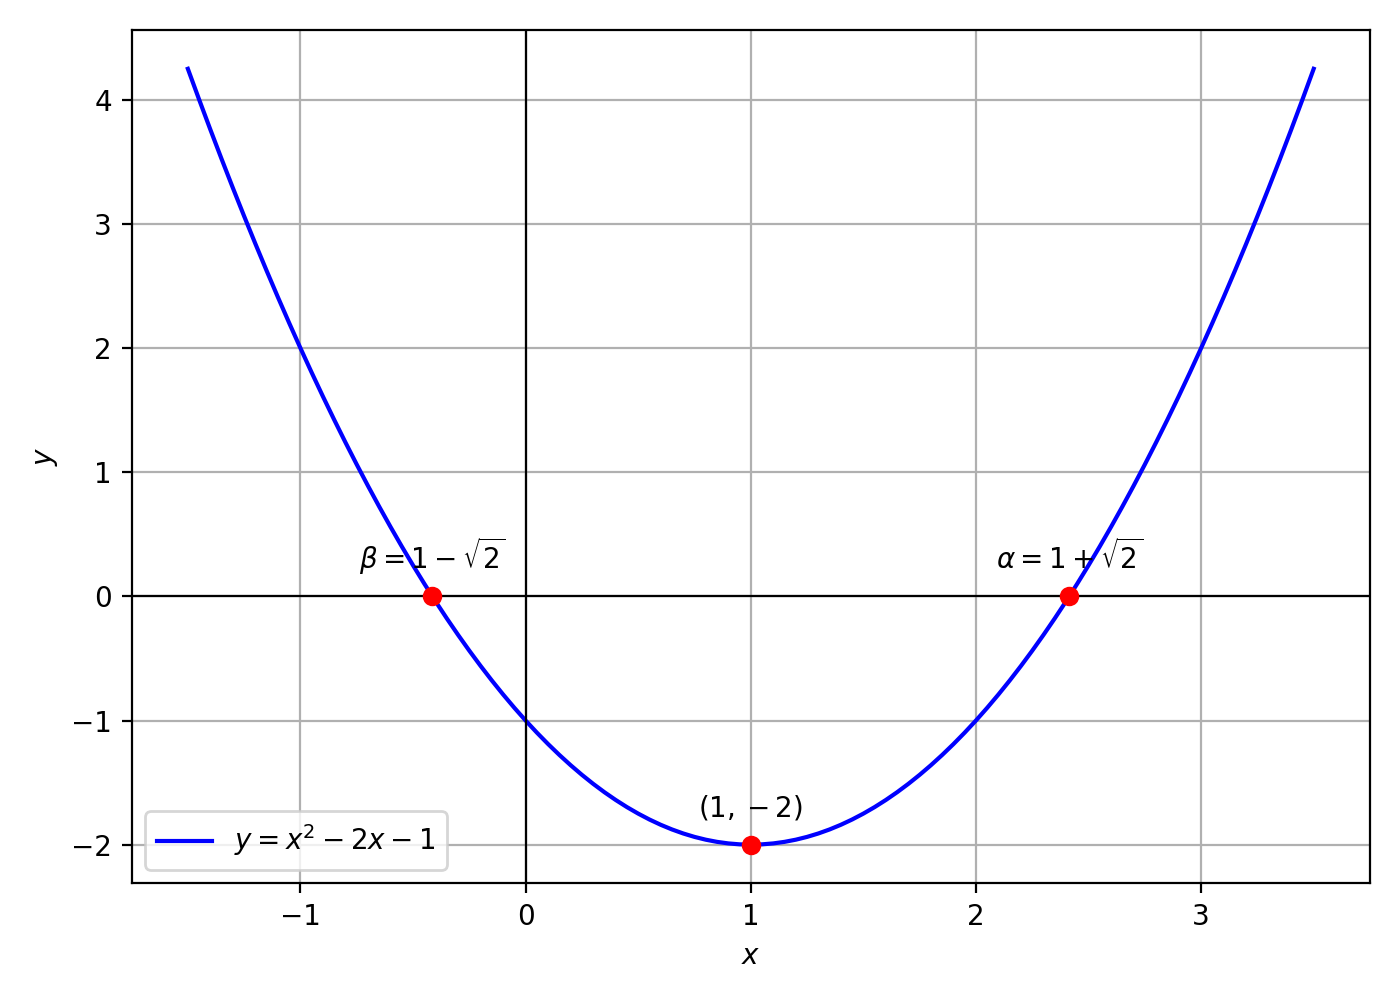
\includegraphics[width=0.6\linewidth]{figs/q21b.png}
	\caption{Graph of $y = x^2 - 2x - 1$ with zeroes $\alpha$ and $\beta$}
	\label{fig:CBSE25S2-q21b}
\end{figure}

\item
In a school, $65\%$ of the students have black eyes, $25\%$ have brown eyes and the rest have blue eyes. A student is chosen at random. Find the probability that the student has (a) blue eyes, (b) brown or black eyes.
\hfill (10, 2025)

\solution
Let $X = 0, 1, 2$ denote black, brown and blue eyes. The probability of blue eyes is $1 - 0.65 - 0.25 = 0.10$, so the pmf is
\begin{table}[H]
	\centering
	\begin{tabular}{|c|c|c|c|}
		\hline
		$x$ & $0$ (black) & $1$ (brown) & $2$ (blue) \\ \hline
		$p_X\brak{x}$ & $0.65$ & $0.25$ & $0.10$ \\ \hline
	\end{tabular}
	\caption{pmf of the eye colour}
	\label{tab:CBSE25S2-q27}
\end{table}
The probability of an event is the sum of the pmf over its outcomes.

\textbf{(a) Blue eyes:}
\begin{align}
	\pr{\text{blue}} = p_X\brak{2} = 0.10
\end{align}
\textbf{(b) Brown or black eyes:}
\begin{align}
	\pr{\text{brown or black}} = p_X\brak{1} + p_X\brak{0} = 0.25 + 0.65 = 0.90
\end{align}
which is also $1 - \pr{\text{blue}} = 0.90$. The following program simulates the eye colours of $10^6$ people and compares the relative frequencies with the pmf
\begin{lstlisting}[frame=single, basicstyle=\rmfamily, escapeinside={(*@}{@*)}]
(*@\makebox[\dimexpr\linewidth-2\fboxsep-2\fboxrule\relax][c]{10/codes/27.c}@*)
\end{lstlisting}
The following code makes a stem plot of the simulated relative frequencies and the pmf, see \figref{fig:CBSE25S2-q27}.
\begin{lstlisting}[frame=single, basicstyle=\rmfamily, escapeinside={(*@}{@*)}]
(*@\makebox[\dimexpr\linewidth-2\fboxsep-2\fboxrule\relax][c]{10/codes/27plot.py}@*)
\end{lstlisting}
\begin{figure}[H]
	\centering
	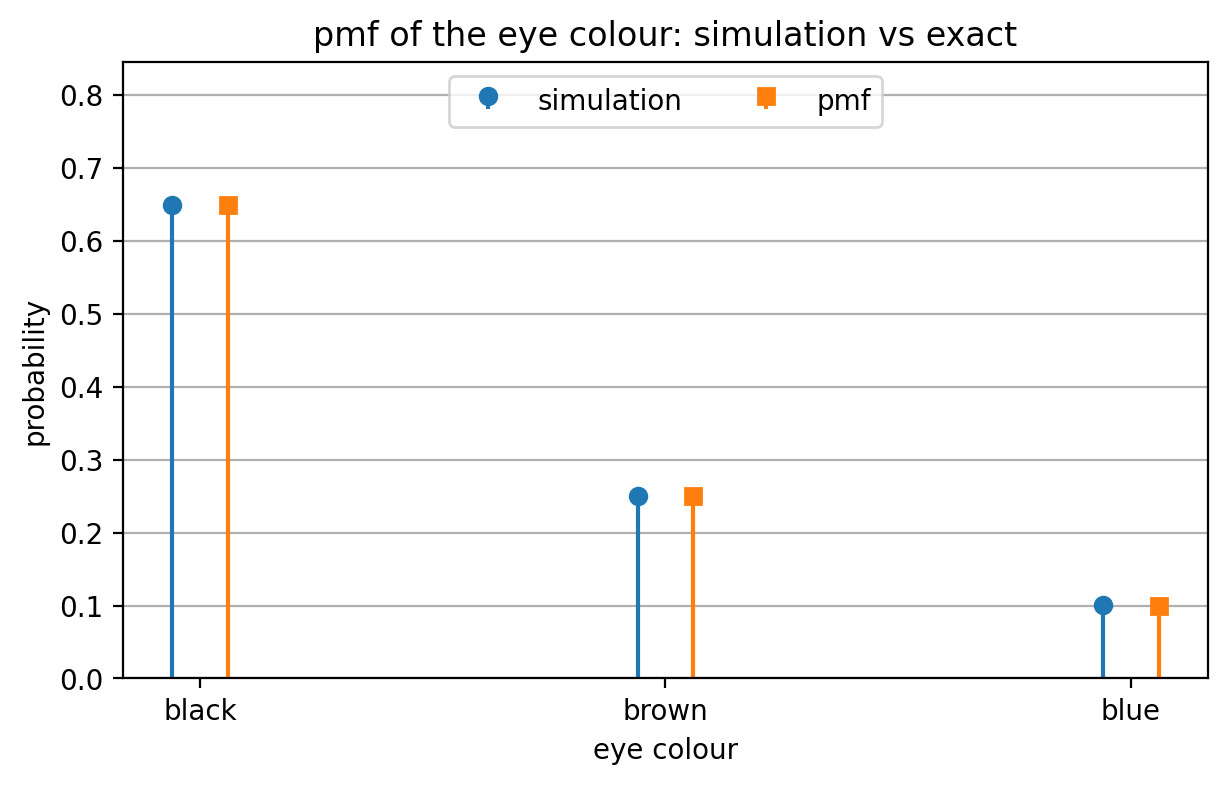
\includegraphics[width=0.8\linewidth]{figs/q27.png}
	\caption{Stem plot of the simulated relative frequencies and the pmf of the eye colour}
	\label{fig:CBSE25S2-q27}
\end{figure}

\item
In the figure, $PC$ is a tangent to the circle at $C$ and $AB$ is a diameter which, when extended, meets the tangent at $P$. If $\angle PCA = 110^\circ$, find $\angle CBA$ and $\angle BCO$.
\hfill (10, 2025)

\solution
Since $AB$ is a diameter, $\angle ACB = 90^\circ$. As $P$ lies beyond $B$,
\begin{align}
	\angle PCA = \angle PCB + \angle BCA \implies \angle PCB = 110^\circ - 90^\circ = 20^\circ
\end{align}
By the tangent--chord theorem, $\angle CAB = \angle PCB = 20^\circ$. In $\triangle ABC$,
\begin{align}
	\angle CBA = 90^\circ - 20^\circ = 70^\circ
\end{align}
Since $OB = OC$, $\triangle OBC$ is isosceles and
\begin{align}
	\angle BCO = \angle CBO = 70^\circ
\end{align}
To plot the figure, take $r = 2$ with $\vec{O} = \myvec{0 \\ 0}$, $\vec{A} = \myvec{-2 \\ 0}$ and $\vec{B} = \myvec{2 \\ 0}$. Since $\angle CAB = 20^\circ$, the central angle is $\angle COB = 2\angle CAB = 40^\circ$, so
\begin{align}
	\vec{C} = r\myvec{\cos 40^\circ \\ \sin 40^\circ} = \myvec{1.53 \\ 1.29}
\end{align}
The tangent at $\vec{C}$ is perpendicular to $\vec{O}\vec{C}$. Writing $\vec{P} = \myvec{p \\ 0}$ on $AB$,
\begin{align}
	\brak{\vec{C}-\vec{O}}^{\top}\brak{\vec{P}-\vec{C}} = 0 \implies p = \frac{r}{\cos 40^\circ} = 2.61
\end{align}
It can be checked that $\brak{\vec{A}-\vec{C}}^{\top}\brak{\vec{B}-\vec{C}} = 0$, so $\angle ACB = 90^\circ$, and that the angle between $\vec{P}-\vec{C}$ and $\vec{A}-\vec{C}$ is $110^\circ$. The following code verifies the solution
\begin{lstlisting}[frame=single, basicstyle=\rmfamily, escapeinside={(*@}{@*)}]
(*@\makebox[\dimexpr\linewidth-2\fboxsep-2\fboxrule\relax][c]{10/codes/29.py}@*)
\end{lstlisting}
The following code generates \figref{fig:CBSE25S2-q29}.
\begin{lstlisting}[frame=single, basicstyle=\rmfamily, escapeinside={(*@}{@*)}]
(*@\makebox[\dimexpr\linewidth-2\fboxsep-2\fboxrule\relax][c]{10/codes/29plot.py}@*)
\end{lstlisting}
\begin{figure}[H]
	\centering
	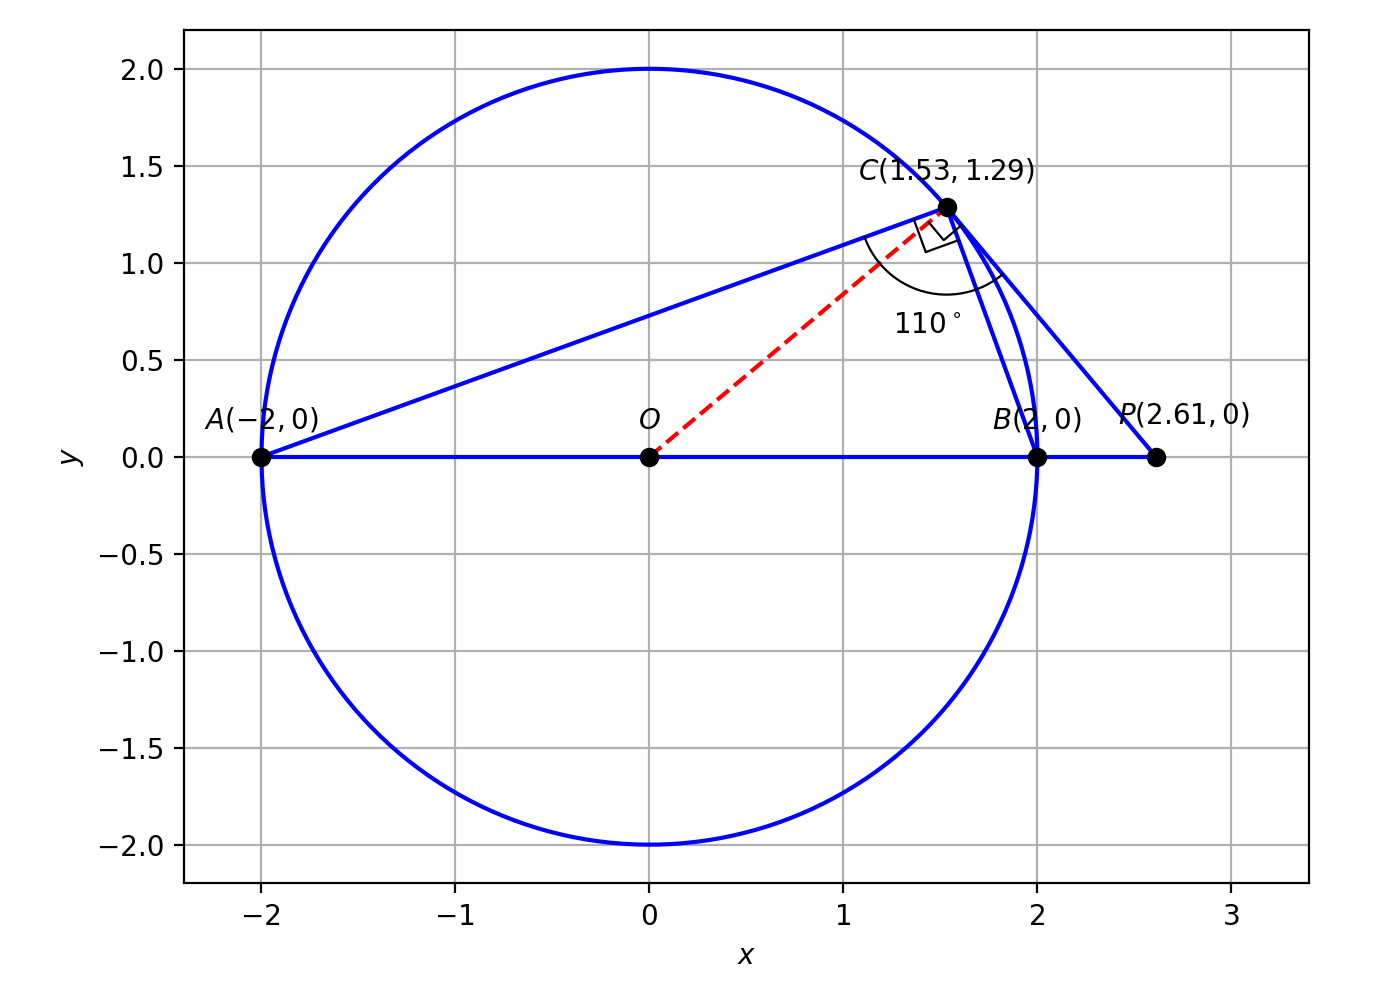
\includegraphics[width=0.6\linewidth]{figs/q29.png}
	\caption{Tangent $PC$ and diameter $AB$, plotted from the coordinates of $\vec{A}$, $\vec{B}$, $\vec{C}$, $\vec{P}$}
	\label{fig:CBSE25S2-q29}
\end{figure}

\item
Find the coordinates of the points which divide the line segment joining $A\brak{-2,2}$ and $B\brak{2,8}$ into four equal parts.
\hfill (10, 2025)

\solution
Let $\vec{A} = \myvec{-2 \\ 2}$ and $\vec{B} = \myvec{2 \\ 8}$. The points that divide $AB$ into four equal parts are
\begin{align}
	\vec{P}_k = \vec{A} + \frac{k}{4}\brak{\vec{B} - \vec{A}}, \quad k = 1, 2, 3
\end{align}
Collecting the terms in $\vec{A}$ and $\vec{B}$,
\begin{align}
	\vec{P}_k = \brak{1 - \frac{k}{4}}\vec{A} + \frac{k}{4}\vec{B} = \myvec{\vec{A} & \vec{B}}\myvec{1 - \frac{k}{4} \\ \frac{k}{4}}
\end{align}
The weights add up to $1$, as they must for a point on the segment. Writing the weights for $k = 1, 2, 3$ side by side as the columns of one matrix,
\begin{align}
	\myvec{\vec{P}_1 & \vec{P}_2 & \vec{P}_3} = \myvec{\vec{A} & \vec{B}}\myvec{\frac{3}{4} & \frac{1}{2} & \frac{1}{4} \\ \frac{1}{4} & \frac{1}{2} & \frac{3}{4}}
\end{align}
and the columns of the product give the three points. Substituting $\myvec{\vec{A} & \vec{B}} = \myvec{-2 & 2 \\ 2 & 8}$,
\begin{align}
	\myvec{\vec{P}_1 & \vec{P}_2 & \vec{P}_3}
	&= \myvec{-2 & 2 \\ 2 & 8}\myvec{\frac{3}{4} & \frac{1}{2} & \frac{1}{4} \\ \frac{1}{4} & \frac{1}{2} & \frac{3}{4}}
	\\
	&= \myvec{-\frac{3}{2} + \frac{1}{2} & -1 + 1 & -\frac{1}{2} + \frac{3}{2} \\ \frac{3}{2} + 2 & 1 + 4 & \frac{1}{2} + 6}
	= \myvec{-1 & 0 & 1 \\ 3.5 & 5 & 6.5}
\end{align}
Hence the points are
\begin{align}
	\vec{P}_1 = \myvec{-1 \\ 3.5}, \quad \vec{P}_2 = \myvec{0 \\ 5}, \quad \vec{P}_3 = \myvec{1 \\ 6.5}
\end{align}
As a check, $\vec{P}_2$ is the mid-point $\frac{\vec{A}+\vec{B}}{2} = \myvec{0 \\ 5}$. The following code verifies the solution
\begin{lstlisting}[frame=single, basicstyle=\rmfamily, escapeinside={(*@}{@*)}]
(*@\makebox[\dimexpr\linewidth-2\fboxsep-2\fboxrule\relax][c]{10/codes/31.py}@*)
\end{lstlisting}
The following code generates \figref{fig:CBSE25S2-q31b}.
\begin{lstlisting}[frame=single, basicstyle=\rmfamily, escapeinside={(*@}{@*)}]
(*@\makebox[\dimexpr\linewidth-2\fboxsep-2\fboxrule\relax][c]{10/codes/31plot.py}@*)
\end{lstlisting}
\begin{figure}[H]
	\centering
	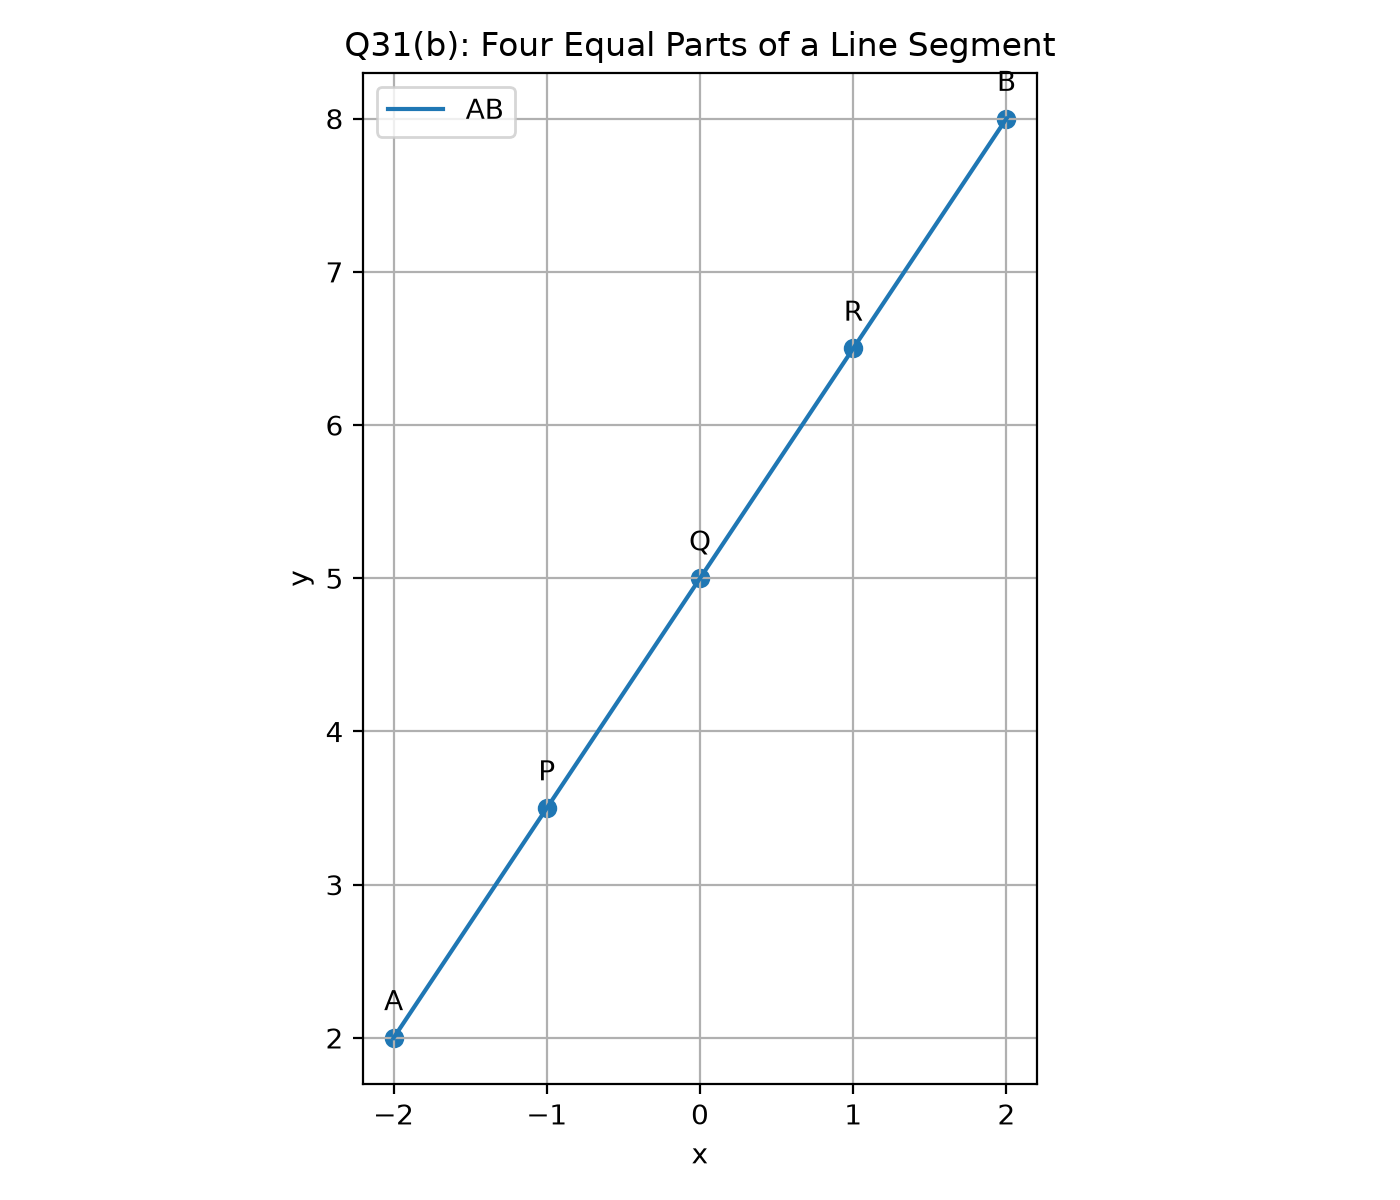
\includegraphics[width=0.5\linewidth]{figs/q31b.png}
	\caption{Division of $AB$ into four equal parts}
	\label{fig:CBSE25S2-q31b}
\end{figure}

\item
The $n^{\text{th}}$ term of an AP is $4$, its common difference is $2$ and the sum of its first $n$ terms is $-14$. Find $n$, the first term, and the sum of the first $20$ terms.
\hfill (10, 2025)

\solution
Let $u\sbrak{n}$ be the unit step function, $u\sbrak{n} = 1$ for $n \ge 0$ and $0$ otherwise. Index the terms from $n = 0$, so that the AP with first term $a$ and common difference $d$ is the causal sequence
\begin{align}
	x\sbrak{n} = \brak{a + nd}\,u\sbrak{n}
\end{align}
with $x\sbrak{0} = a$. The running sum $y\sbrak{n} = x\sbrak{0} + \cdots + x\sbrak{n}$ is the convolution $y = x * u$, so in the $z$-domain $Y\brak{z} = X\brak{z}U\brak{z}$. Using the transform pairs
\begin{align}
	u\sbrak{n} \xleftrightarrow{\ \mathcal{Z}\ } \frac{1}{1 - z^{-1}}, \quad
	n\,u\sbrak{n} \xleftrightarrow{\ \mathcal{Z}\ } \frac{z^{-1}}{\brak{1 - z^{-1}}^2}
\end{align}
the transform of the AP is
\begin{align}
	X\brak{z} &= \frac{a}{1 - z^{-1}} + \frac{d\,z^{-1}}{\brak{1 - z^{-1}}^2}
	\\
	\implies Y\brak{z} &= \frac{a}{\brak{1 - z^{-1}}^2} + \frac{d\,z^{-1}}{\brak{1 - z^{-1}}^3}
\end{align}
From the pairs
\begin{align}
	\brak{n+1}u\sbrak{n} \xleftrightarrow{\ \mathcal{Z}\ } \frac{1}{\brak{1 - z^{-1}}^2}, \quad
	\frac{n\brak{n+1}}{2}u\sbrak{n} \xleftrightarrow{\ \mathcal{Z}\ } \frac{z^{-1}}{\brak{1 - z^{-1}}^3}
\end{align}
the inverse transform gives the sum of the first $n+1$ terms,
\begin{align}
	y\sbrak{n} = \brak{n+1}a + \frac{n\brak{n+1}}{2}d, \quad n \ge 0
\end{align}
Let $m$ be the index of the last term, so that the number of terms is $m + 1$. Here $d = 2$, $x\sbrak{m} = 4$ and $y\sbrak{m} = -14$. From $x\sbrak{m} = a + 2m = 4$ we get $a = 4 - 2m$, and
\begin{align}
	y\sbrak{m} = \brak{m+1}\brak{4 - 2m} + m\brak{m+1} &= \brak{m+1}\brak{4 - m} = -14
	\\
	\implies m^2 - 3m - 18 &= 0 \implies \brak{m-6}\brak{m+3} = 0
\end{align}
Since $m \ge 0$, $m = 6$, so the number of terms is $m + 1 = 7$ and $a = 4 - 12 = -8$. The sum of the first $20$ terms is $y\sbrak{19}$,
\begin{align}
	y\sbrak{19} = 20\brak{-8} + \frac{19 \cdot 20}{2}\brak{2} = -160 + 380 = 220
\end{align}
The following code verifies the solution
\begin{lstlisting}[frame=single, basicstyle=\rmfamily, escapeinside={(*@}{@*)}]
(*@\makebox[\dimexpr\linewidth-2\fboxsep-2\fboxrule\relax][c]{10/codes/32a.py}@*)
\end{lstlisting}

\item
A man lent part of his money at $10\%$ per annum and the rest at $15\%$ per annum. His yearly interest was \rupee 1900. Had he interchanged the two rates, he would have earned \rupee 200 more. Find the two amounts.
\hfill (10, 2025)

\solution
Let $x$ and $y$ be the amounts lent at $10\%$ and $15\%$. Then
\begin{align}
	0.10x + 0.15y &= 1900 \\
	0.15x + 0.10y &= 2100
\end{align}
The augmented matrix of $\vec{A}\vec{x} = \vec{b}$ is $\myvec{\vec{A} & \vec{b}}$. Using Gaussian elimination (Gauss--Jordan row reduction),
\begin{align}
	\myvec{0.10 & 0.15 & 1900 \\ 0.15 & 0.10 & 2100}
	&\xleftrightarrow[]{R_1 \leftarrow 10R_1}
	\myvec{1 & 1.5 & 19000 \\ 0.15 & 0.10 & 2100}
	\\
	&\xleftrightarrow[]{R_2 \leftarrow R_2 - 0.15R_1}
	\myvec{1 & 1.5 & 19000 \\ 0 & -0.125 & -750}
	\\
	&\xleftrightarrow[]{R_2 \leftarrow R_2/\brak{-0.125}}
	\myvec{1 & 1.5 & 19000 \\ 0 & 1 & 6000}
	\\
	&\xleftrightarrow[]{R_1 \leftarrow R_1 - 1.5R_2}
	\myvec{1 & 0 & 10000 \\ 0 & 1 & 6000}
\end{align}
Both $\vec{A}$ and $\myvec{\vec{A} & \vec{b}}$ have two non-zero rows, so
\begin{align}
	\rank\brak{\vec{A}} = \rank\myvec{\vec{A} & \vec{b}} = 2 = \text{number of unknowns}
\end{align}
Hence the system is consistent with a unique solution,
\begin{align}
	\vec{x} = \myvec{x \\ y} = \myvec{10000 \\ 6000}
\end{align}
The amounts are \rupee 10000 at $10\%$ and \rupee 6000 at $15\%$. The following code verifies the solution
\begin{lstlisting}[frame=single, basicstyle=\rmfamily, escapeinside={(*@}{@*)}]
(*@\makebox[\dimexpr\linewidth-2\fboxsep-2\fboxrule\relax][c]{10/codes/34.py}@*)
\end{lstlisting}

\item
\textbf{Case study (lighthouse).} A lighthouse $AB$ is $50$ m high. From its top $B$, the angles of depression of a ship at $P$ and, after some time, at $Q$ are $30^\circ$ and $45^\circ$ respectively, with $P$, $Q$, $A$ on the same line.
\hfill (10, 2025)
% TODO: part (ii) of the paper is not included - its exact wording was not verified


\solution
Take the foot of the lighthouse as the origin, $\vec{A} = \myvec{0 \\ 0}$ and $\vec{B} = \myvec{0 \\ 50}$, with the ground along the $x$-axis, $\vec{e}_2^{\top}\vec{x} = 0$. The line of sight from $\vec{B}$ with angle of depression $\theta$ has direction vector $\vec{m} = \myvec{\cos\theta \\ -\sin\theta}$ and meets the ground when
\begin{align}
	\vec{e}_2^{\top}\brak{\vec{B} + \lambda\vec{m}} = 0
	\implies \lambda = -\frac{\vec{e}_2^{\top}\vec{B}}{\vec{e}_2^{\top}\vec{m}} = \frac{50}{\sin\theta}
\end{align}
For $\vec{Q}$ ($\theta = 45^\circ$) and $\vec{P}$ ($\theta = 30^\circ$),
\begin{align}
	\vec{Q} &= \vec{B} + 50\sqrt{2}\cdot\frac{1}{\sqrt{2}}\myvec{1 \\ -1} = \myvec{50 \\ 0}
	\\
	\vec{P} &= \vec{B} + 100\cdot\frac{1}{2}\myvec{\sqrt{3} \\ -1} = \myvec{50\sqrt{3} \\ 0}
\end{align}
\textbf{(i)} The distance $QA$ is
\begin{align}
	QA = \norm{\vec{Q}-\vec{A}} = 50 \text{ m}
\end{align}
\textbf{(iii)(a)} The distance moved from $P$ to $Q$ is
\begin{align}
	PQ = \norm{\vec{P}-\vec{Q}} = 50\brak{\sqrt{3} - 1} \approx 36.60 \text{ m}
\end{align}
\textbf{(iii)(b)} The ship covers $QA = 50$ m $= 0.05$ km in $10$ minutes $= \frac{1}{6}$ h, so
\begin{align}
	\text{Speed} = \frac{0.05}{1/6} = 0.3 \text{ km/h}
\end{align}
The following code verifies the solution
\begin{lstlisting}[frame=single, basicstyle=\rmfamily, escapeinside={(*@}{@*)}]
(*@\makebox[\dimexpr\linewidth-2\fboxsep-2\fboxrule\relax][c]{10/codes/38.py}@*)
\end{lstlisting}
The following code generates \figref{fig:CBSE25S2-q38}.
\begin{lstlisting}[frame=single, basicstyle=\rmfamily, escapeinside={(*@}{@*)}]
(*@\makebox[\dimexpr\linewidth-2\fboxsep-2\fboxrule\relax][c]{10/codes/38plot.py}@*)
\end{lstlisting}
\begin{figure}[H]
	\centering
	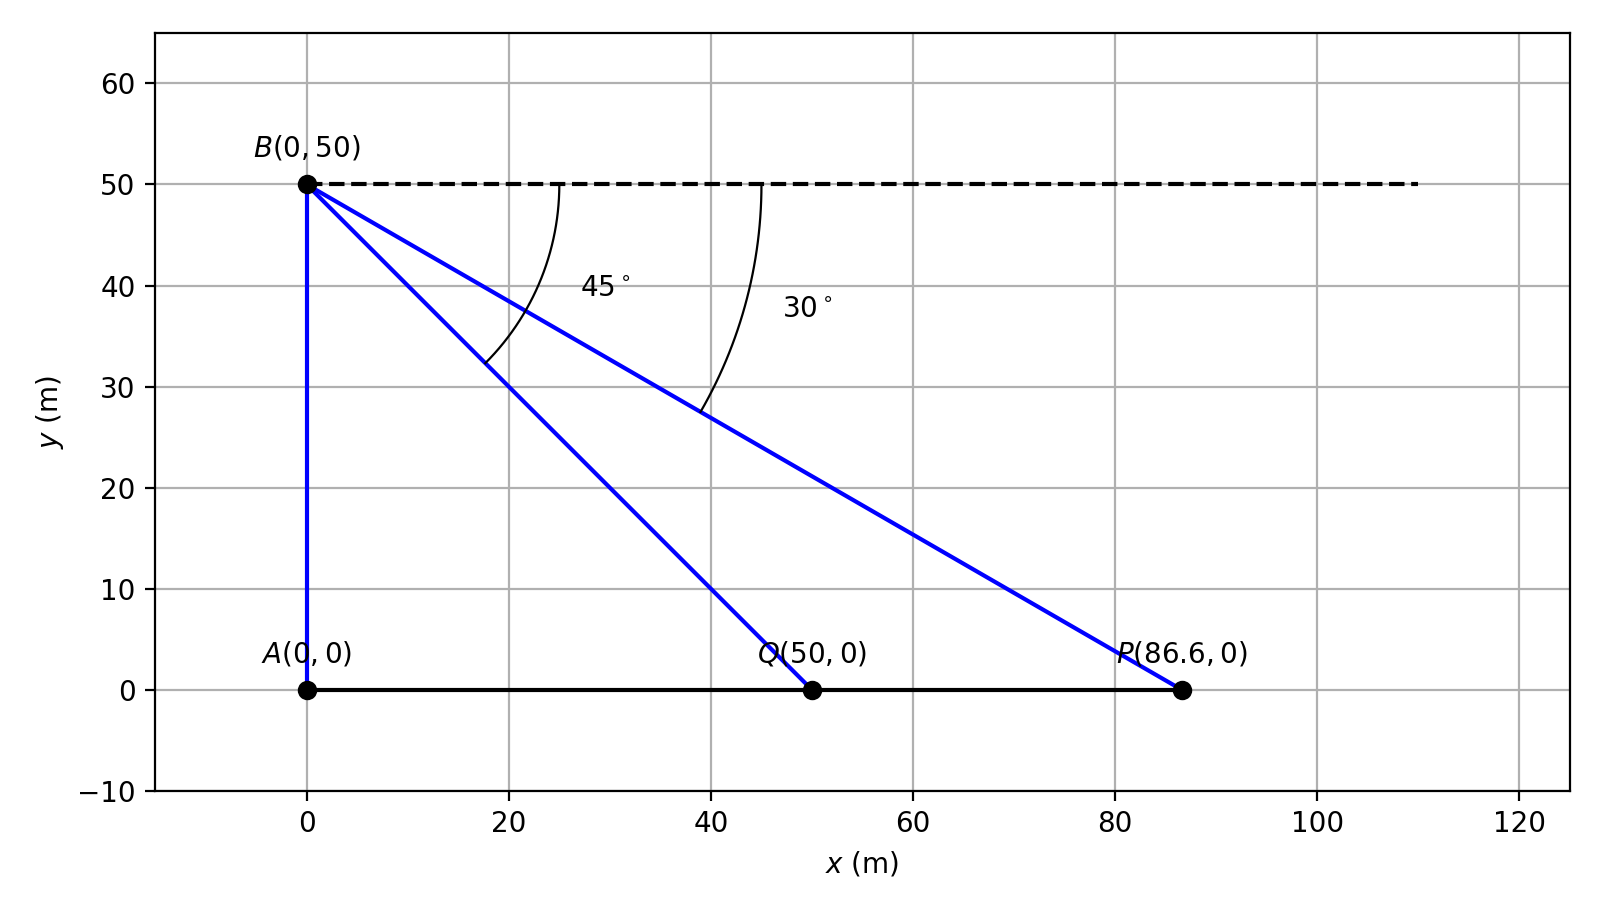
\includegraphics[width=0.8\linewidth]{figs/q38.png}
	\caption{Lighthouse $AB$ and ship positions $P$, $Q$, plotted from coordinates}
	\label{fig:CBSE25S2-q38}
\end{figure}

\end{enumerate}
